\documentclass[10pt,twocolumn,letterpaper]{article}
\usepackage[review]{cvpr}
\usepackage{cuted}
\usepackage{microtype}
\definecolor{cvprblue}{rgb}{0.21,0.49,0.74}
\usepackage[pagebackref,breaklinks,colorlinks,allcolors=cvprblue]{hyperref}
\usepackage[capitalize,noabbrev]{cleveref}
\def\confName{CVPR}
\def\confYear{2027}
\graphicspath{{figures/}}
\title{Same Parts, Different Arrangements\\Matched Edits for Budgeted Anomaly Inspection}
\author{Anonymous}
\hypersetup{pdftitle={Same Parts, Different Arrangements},pdfauthor={},
            pdfsubject={Anonymous CVPR 2027 submission}}

\begin{document}
\raggedbottom
\maketitle
\begin{strip}
\centering
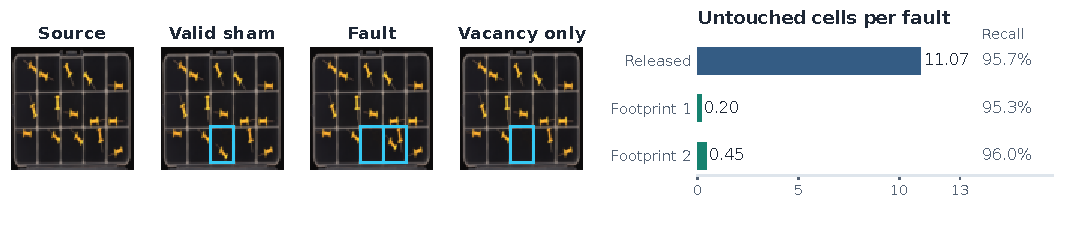
\includegraphics[width=\linewidth]{inspection_teaser.pdf}
\captionsetup{hypcap=false}
\captionof{figure}{\textbf{A matched test for where to look after an alert.} We move the same intact pin the same distance within its compartment or into an occupied neighbor. Vacancy-only retains the same source fill. On 138 photos with parts re-extracted from edited RGB, the released composition branch detects every fault. Two footprint-supervised adaptations retain every fault alert and reduce the number of untouched compartments queued at a development-calibrated target recall of 95\%. The bars show test costs and achieved recall.}
\label{fig:teaser}
\captionsetup{hypcap=true}
\end{strip}

\begin{abstract}
An anomaly detector can flag the right scene and still send an inspector to many intact parts. The released SALAD composition branch detects all 138 matched pushpin placement faults, ranks each above its valid sham, and achieves 98.2\% affected-compartment AUROC. Its best two cells often suffice, but a validation-calibrated queue for high recall includes 11.07 of 13 untouched cells per fault after re-extracting parts from RGB. Adapting the head on rule-aware training edits with footprint supervision reduces that queue to 0.20--0.45 untouched cells at 95.3--96.0\% target recall across two seeds and retains all fault detections. A paired continuation using the original synthetic families also reduces queue size when its class-wide control reproduces the released response. Valid-sham alert rates rise in one seed relative to the release. A fresh liquid--label test on 89 bottles identifies which SALAD branch can distinguish a mismatch from an equally edited valid label. Matched controls connect map supervision and branch choice to the work an inspector actually faces.
\end{abstract}

\section{Introduction}
A tray with a missing pin and a doubled pin has the right inventory. A detector should flag the tray and point to the two compartments that need attention. The released SALAD composition branch \cite{fucka2025} detects all 138 such rearrangements of MVTec LOCO photographs \cite{bergmann2022}. Its two highest-scoring cells also find both targets on most scenes. If the inspector needs to find nearly every target, however, a single threshold can produce a much longer queue. We measure when that happens and how a researcher can shorten it.

We use the same intact pin for a valid move inside a cell and an invalid move into an occupied neighbor, matching displacement and paste support. The vacancy-only control preserves the missing part of the fault and isolates the effect of adding a pin in the occupied cell. The intervention gives an exact pair of cells for inspection. This lets us test a training choice that is hard to evaluate on naturally occurring logical faults. SALAD marks all instances of an inserted class because, for example, the extra screw in an unordered bag can be interchangeable with the original screws \cite{fucka2025}. Our compartments specify which locations violate the rule. We can assign that supervision while holding the synthetic maps fixed.

We make three comparisons. First, we replay the released model, show its performance at fixed ranks and thresholds, and compare two target policies with the same initial weights and input edits. The largest savings come from footprint targets during rule-aware adaptation. Second, we evaluate the released full system on the same pushpins and on a different rule in juice bottles. The valid shams expose strong RGB sensitivity on pushpins, while the global appearance branch supplies useful evidence about the liquid--icon relation. Third, we refit a graph readout to test whether a strong response to degree-preserving switches depends on the degrees presented to the query-masked model.

\section{Related work}
MVTec LOCO defines logical defects through explicit scene constraints and introduces saturated per-region overlap to accommodate ambiguity in localization \cite{bergmann2022}. Component methods use attributes, correspondence, reconstruction, or executable rules \cite{liu2023,peng2025,zhang2026logico,ji2026}. SALAD learns from composition maps alongside two RGB branches \cite{fucka2025,batzner2024}. LogicAL uses synthetic logical defects to learn localization \cite{zhao2024}. We use matched interventions to compare supervision and readout policies and measure the resulting queue at a cutoff fixed on development. The labels in the audit identify actions an inspector can take under a specified rule.

Matched composition tests have also been used in vision--language evaluation, where captions can retain words while changing their relations \cite{thrush2022}. Here the matched variants retain a reference region or query across inputs. We use both valid shams and a targeted removal to distinguish evidence of the intended violation from evidence of compositing or a vacancy. For graphs, target-link masking and degree-sensitive performance have been studied in link prediction \cite{zhu2024spot}. Our graph intervention measures how masking changes the signal available even when the two full graphs have identical degree sequences.

\section{Matched edits and inspection decisions}
\label{sec:design}
\paragraph{Photographs and controls.}
We use all 138 previously established held-out normal pushpin photographs. The published rule assigns one pin to each of 15 compartments \cite{bergmann2022}. Using the released class mask and immediate RGB halo, we cut out an intact pin at $256{\times}256$ and translate it without resampling. The sham leaves one pin in each cell. The fault leaves the source cell empty and doubles the pin in an occupied face-adjacent cell. Both use the same cutout, background fill and displacement magnitude. Collision, divider clearance and background agreement are checked before scoring. A fourth variant only fills the vacated support. The vacated and recipient cells are the fault targets. The former alone is the vacancy-only target.

The oracle interface uses the released labels and moves the pin mask directly. The extracted interface independently segments each RGB variant, including the original, with a separately fitted U-Net trained on official normal training data. Both use the same SALAD composition weights. These paths let us check that a result survives re-segmentation of the composites. The released model consumes a six-channel one-hot map and concatenates it with the autoencoder's softmax reconstruction. The discriminative U-Net returns a sigmoid map.

\paragraph{Scene gate and inspection queue.}
For a raw predicted map $S_i$ on image $i$, a scene alerts if its maximum exceeds a strict split-conformal 10\% cutoff from 69 untouched validation photos \cite{bates2023}. For an alert, each registered cell $e$ has a score $g(S_i|_e)$, the maximum by default. We queue cells at or above $t_c$. The queue is empty if the scene is clear. For the two targets $T_i$ we measure
\[
 R=\frac{1}{2n}\sum_i|Q_i\cap T_i|,\qquad
 C=\frac{1}{n}\sum_i|Q_i\setminus T_i|.
\]
We fit $t_c$ separately for each map and input path as the highest threshold attaining 95\% target recall on 69 matched validation faults. A gated-out scene contributes two misses. A second cutoff constrains development cost to at most 0.5 untouched cells per fault. We also report the fraction with both targets in the top two or three and the rank of the second target, with cell index breaking exact ties.

The primary contrast is the difference in $C$ between target policies on extracted maps. We locked a useful reduction of one cell, a paired interval excluding zero, at least 90\% achieved target recall and at most five points below the control, and at least 95\% fault and vacancy scene recall with at most three points lost. We also guard against more than five points of extra sham alerts relative to the paired control. We require a competent class-wide control on development for mechanism claims, including at least 90\% cell AUROC. Uncertainty uses 4,000 bootstrap draws by original photo, carrying all variants, policies and input paths together. The two seeds and two fixed photo halves check stability. The intervals condition on the fitted models and cutoffs.

\paragraph{Absolute scores and paired response.}
The inspection decisions use only the edited map. For diagnosis we also compare the same cells in the source and compute $|S_i^{\rm edit}-S_i^{\rm source}|$. We summarize maxima, upper quantiles and changed pixel area on the same 13 unaffected cells across fault, sham and vacancy. A low-FPR region analogue of AU-sPRO \cite{bergmann2022,fucka2025} counts a cell as recovered when its score crosses a common threshold. We integrate target-cell recall over pooled false cell rate from 0 to 0.05 and divide by 0.05. All cells in the valid source and sham plus untouched fault cells are negatives. A fault-only version removes the clean variants. This uses binary saturation at the cell level. The inspection endpoint additionally specifies how to choose the cutoff and includes the separate scene gate.

\section{Choose supervision for the inspection budget}
\label{sec:results}
\begin{table*}[t]
\centering
\caption{\textbf{Stand-alone pushpin inspection after re-extraction from edited RGB.} All rows use the same 138 originals and show scene alert counts. Top 2 is recovery of both affected cells. Marks to both is the mean rank of the second target. Recall and untouched marks use the locked 95\% development queue. Region area is the normalized cell analogue of AU-sPRO at FPR $\leq0.05$, in percent. Fine-tunes have identical inputs within each seed.}
\label{tab:inspection}
\small
\setlength{\tabcolsep}{5pt}
\begin{tabular}{lccccrrr}
\toprule
Map and compartment score & Src. / Sham & Fault / Vac. & Top 2 (\%) & Marks to both & Recall (\%) & Untouched & Reg. area \\
\midrule
Released, max & 5 / 7 & 138 / 138 & 77.5 & 2.43 & 95.7 & 11.07 & 81.6 \\
Released, 99th pct. & 5 / 7 & 138 / 138 & 87.0 & 2.32 & 96.0 & 11.41 & 77.3 \\
\midrule
Class-wide, seed 1 & 12 / 19 & 138 / 138 & 0.0 & 15.00 & 97.1 & 13.00 & 39.3 \\
Footprint, seed 1 & 6 / 9 & 138 / 138 & 87.7 & 2.13 & 95.3 & 0.20 & 96.3 \\
\midrule
Class-wide, seed 2 & 19 / 22 & 138 / 138 & 0.0 & 15.00 & 96.4 & 13.00 & 39.4 \\
Footprint, seed 2 & 21 / 20 & 138 / 138 & 74.6 & 2.28 & 96.0 & 0.45 & 89.6 \\
\bottomrule
\end{tabular}

\end{table*}

\paragraph{What the released map already does well.}
The official composition branch detects all 138 faults and all vacancies on both interfaces. It ranks the fault above the valid sham for every pair. The exact 95\% interval for 138/138 is 97.4--100\%. On oracle labels, affected-cell AUROC rises from 48.6\% in the source to 98.2\% after the fault. Ranking by maximum absolute change reaches 98.4\%. On extracted maps, both targets are among the top two in 77.5\% of faults and among the top three in 94.2\%. The second target takes 2.43 marks on average. With a hard budget of two, the development-selected 99th percentile improves both-target recovery to 87.0\% ($+9.4$ points [4.3, 14.5]) using the same scene gate and weights.

\paragraph{Where the budget changes the choice.}
At the 95\% development recall cutoff, the released maximum reaches 95.7\% target recall on extracted faults while queuing 11.07 untouched cells per fault. Using the 99th percentile increases both-target recovery at rank two, but queues 11.41 untouched cells at 96.0\% achieved recall. A lower-cost threshold gives 81.9\% recall with 0.30 untouched cells using the maximum, and 75.7\% with 0.17 using the 99th percentile. One ranking can be preferable for two suggestions and another for a global cutoff. The remaining readouts and 98\% calibration are in the supplement.

\paragraph{What moved and what alerted.}
A pixel changes by at least 0.5 in 90.3\% of untouched oracle cells in the relocation, 2.9\% in the vacancy-only control, and 0.7\% in the sham. The relocation statistic is 89.4\% after extraction. Across the actual area of those untouched cells, 5.4\% of pixels change that much on either interface. The extracted mean within-cell maximum, 99th and 95th percentiles of the change are 0.777, 0.706 and 0.578. The response has strong peaks dispersed across cells, with much less total area affected. Both oracle source and sham alert on 31/138, with two new and two cleared alerts. Extraction gives five source and seven sham alerts, including two new and zero cleared. An explicit one-pin-per-cell rule has zero sham alerts and detects all faults on both inputs. It uses the rule supplied by the application.

\begin{figure*}[t]
\centering
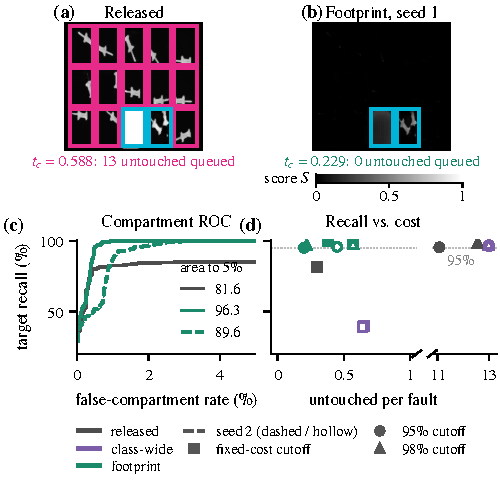
\includegraphics[width=\linewidth]{guidance_maps.pdf}
\caption{\textbf{Raw scores support the inspection decision.} The extracted fault shown is the median released fault--sham score difference. Cyan boxes are targets. Orange boxes are untouched cells at or above the locked cutoff. A dashed cyan box denotes a missed target when present. The region curve pools fault, sham and source cells at common thresholds. Its area also favors the footprint head, while the locked queue measures the actual cell cost.}
\label{fig:maps}
\end{figure*}

\paragraph{Change the spatial target.}
SALAD \S3.4 defines the positive region for insertion as every pixel of the inserted class \cite{fucka2025}. The pinned \texttt{copy\_label\_diff\_img} first overwrites a rotated donor footprint, then returns the entire resulting class plane as the discriminative mask. \texttt{copy\_and\_change} takes the union with the same-image relabel mask. The training loop uses five times mean sigmoid focal plus mean L1 for the anomaly map, and multiclass focal plus Dice against the clean composition for reconstruction. We preserve the relabel targets. We change the insertion portion from the class plane to the recorded donor footprint. For relocations both arms include the old footprint, and the class-wide arm additionally marks all pins in the resulting map while the footprint arm marks the pasted pin. Vacancies share the same old-footprint target. Both give valid shams a zero target.

Each fine-tune starts from the same released composition weights and freezes the reconstruction autoencoder. Each batch has two clean maps, one SALAD-style synthetic edit and one rule-aware training variant drawn from the official training photos. We use 800 Adam steps and the final checkpoint. All inputs, edit identities, steps, loss coefficients and pixel weights are shared. For seed 1 the mean relocation mask has 3,823 positive pixels with class-wide supervision and 461 with footprint supervision. The masks change the amount and placement of positive loss. The experiment estimates their joint policy effect. Training uses the known rule to make matched variants. At test time it uses a learned map, registered cell boundaries and the two calibrated thresholds.

\paragraph{Footprints shorten high-recall queues.}
On extracted maps the two footprint heads reduce untouched marks versus the release from 11.07 to 0.20 and 0.45, at 95.3\% and 96.0\% target recall (\cref{tab:inspection}). The paired reductions are 10.88 [10.12, 11.56] and 10.62 [9.86, 11.31] marks. All 138 faults and vacancies still alert. The first seed yields nine valid-sham alerts and the second yields 20, versus seven for the release. The oracle path shows similar queue savings. At the development budget of 0.5 untouched cells, the footprint heads reach 100.0\% and 98.2\% target recall at achieved costs of 0.38 and 0.57, versus 81.9\% at 0.30 for the release. At an equal realized cost of 0.50 marks in a descriptive test sweep, recall is 82.6\% for the release and 100.0\% and 97.1\% for the footprint heads. At rank two, seed 2 falls below the release. The high-recall threshold benefit repeats across the two fixed halves. The low-FPR region area improves from 81.6\% to 96.2\% and 89.6\%. It detects the localization gain. The matched edits additionally separate relocation from vacancy and test whether the training target can change the deployment cost.

\paragraph{What the paired fine-tunes identify.}
The class-wide rule-aware heads preserve all scene detections and assign large changes to all untouched cells, but their affected-cell AUROC falls to about 49\%. They fail the locked localization competence check. Within this adaptation recipe, changing only the target produces a large difference in both seeds, with 13.00 untouched marks under the class-wide policy. The comparison to the released model measures the practical gain of the entire adaptation. It cannot allocate that gain solely to the mask change.
A separately locked continuation uses the original synthetic edit families alone. Its class-wide seed 2 passes development competence (97.3\% extracted cell AUROC), ranks targets at 98.1\% test AUROC and produces a large change in 88.8\% of untouched cells. In that pair, footprint supervision reduces the fraction to 1.3\% and the queue from 11.50 to 7.07, a paired reduction of 4.43 marks [3.72, 5.14] at 96.0\% and 95.3\% target recall. Both heads detect all faults and vacancies, with 18 and 20 sham alerts. Seed 1 gives a similar queue reduction and misses the development AUROC floor. This isolates an effect of insertion targets during a continuation that reproduces the broad response in one competent control. The fine-tune with rule-aware examples achieves the lowest queues.


\section{Branch choice under a second rule}
\label{sec:transfer}
We replayed full SALAD with the released weights. The local teacher, student and appearance autoencoder receive bilinearly resized RGB with ImageNet normalization. The composition branch receives one-hot maps. The global Gaussian branch pools the first 384 RGB student channels over the scene and over classes defined by the supplied maps. We estimate the pinned normal statistics on official training and validation splits. The fusion sums the normalized appearance maximum, normalized composition maximum and Gaussian score \cite{fucka2025}. The Gaussian branch has a scalar output. We keep its spatially pooled evidence separate from the two output maps.

On 91 native logical pushpin faults and 138 native good photographs, fusion reproduces 100.0\% logical AUROC. On the matched composites it scores every fault above its sham, yet alerts on 130/138 extracted-path shams and 75/138 sources. There are 55 newly alerted shams. The local appearance branch alone alerts on 128 shams and nine sources. Its inputs include the compositing changes in both arms. The matched sham reveals an operating cost of RGB fusion on these composites that the native AUROC does not quantify.

\begin{figure}[t]
\centering
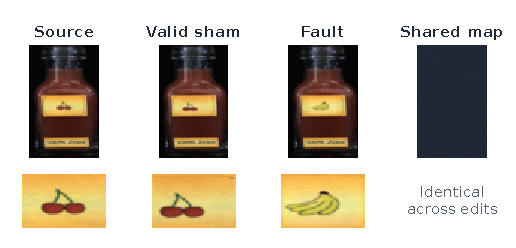
\includegraphics[width=\columnwidth]{juice_rule.pdf}
\caption{\textbf{Juice bottle transfer.} A same-icon transplant preserves the liquid--label rule. An intact different icon violates it. Both edits use the same crop geometry and edge blend. The composition branch receives the same labels and returns the same map for all three.}
\label{fig:juice}
\end{figure}

\begin{table*}[t]
\centering
\caption{\textbf{A second rule on 89 held-out juice bottles.} Counts use separate 10\% normal validation cutoffs. Wins compare fault and sham scores within each original, with half credit for ties. The fault-minus-sham alert gap is in percentage points. Intervals resample originals with all their variants.}
\label{tab:juice}
\small
\begin{tabular}{lrrrcc}
\toprule
Branch & Src. & Sham & Fault & Pair wins (\%) & Alert gap (pp) \\
\midrule
Composition & 4 & 4 & 4 & 50.0 [50.0, 50.0] & +0.0 [+0.0, +0.0] \\
Local appearance & 6 & 28 & 25 & 38.2 [28.1, 48.3] & -3.4 [-12.4, +5.6] \\
Global appearance & 9 & 14 & 89 & 100.0 [100.0, 100.0] & +84.3 [+76.4, +91.0] \\
Full fusion & 7 & 18 & 89 & 100.0 [100.0, 100.0] & +79.8 [+70.8, +87.6] \\
\bottomrule
\end{tabular}

\end{table*}

\paragraph{Liquid and icon.}
MVTec LOCO specifies that the upper label icon must correspond to the liquid \cite{bergmann2022}. We retain 89 of 94 eligible-split normal originals after score-free crop and matching checks. We paste intact icons from a disjoint fixed training bank into the same upper-label support. A same-type icon is a valid sham and another type is a fault. Both use the same relative donor offset, blending, and recipient footprint. Their blended mean RGB changes differ by at most half a digital level over that footprint. The liquid, bottle and released label map are fixed. Eligibility and donor assignments are frozen before scoring. This is an independent rule and a different input intervention. Intervals group by original bottle conditional on the donor bank.

The global RGB branch scores all 89 mismatches above their shams and alerts on all faults, with 14 valid-sham alerts (\cref{tab:juice}). Fusion also detects all faults and alerts on 18 shams. The composition branch ties exactly. The local RGB map puts the upper label first among five bottle regions on 74.2\% of faults, 85.4\% of shams and 5.6\% of originals. Its scene maximum alerts on 25 faults and 28 shams. For this rule, the global input supplies the more selective scene evidence. Local map guidance and scene selectivity can favor different branches. The transfer test evaluates branch choice and the matched audit, with pushpin target adaptation evaluated only on pushpins.

\section{Graph check on response evidence}
\label{sec:graph}
We retain the geometry and degree-preserving GlaS and HVSMR switches, with the original donor folds \cite{glas2017,pace2024}. In GlaS, adding local gland spacing to typed centroid distance improves edited-state AUROC by 15.3 points [11.0, 20.3]. The gain persists on extra length-matched switches and under the stricter joint matching of raw and local distances ($+16.8$ [11.3, 23.0]). These tiers reuse donors. They identify changed pairs with no pathological labels.

For a masked link predictor with logit $z_e$ and observed state $a_e$, the Bernoulli loss is $\operatorname{softplus}(z_e)-a_e z_e$. Changing the observed bit can move the loss with fixed conditional evidence. The pair MLP receives unchanged geometry and roles, giving an invariant probability by construction. A query-masked neighborhood model has another route. At an endpoint of the query its input degree is $d_i-a_e$, so degree-preserving switches change that degree by $-\Delta a_e$. SpotTarget studies target-link inclusion, exclusion and degree effects in link prediction \cite{zhu2024spot}. Here the target is excluded in both states, and the switch changes the degree supplied by the resulting graph.

The original GNN recovers 87.5\% of edits at four reviewed pairs when ranked by absolute probability change. Holding its degree inputs and degree-scaled pooling fixed reduces that to 33.7\%, a sensitivity test on hybrid inputs. We refit with mean neighborhood aggregation and no explicit degree inputs on the same four GlaS folds. The refit attains 95.7--98.2\% normal-link development AUROC and beats the intercept in all folds. Its top-four recovery is 46.6\%, 40.9 points lower [32.8, 49.8] than the original. Both variants use the same edit targets. Mean aggregation still allows indirect cues from neighborhood contents and emptiness. The clamp and refit support a dependence on the degree route without treating recovery of known graph edits as clinical validity.

\section{Scope}
The strongest deployment result concerns two marked compartments in a registered tray. Both seeds improve the calibrated high-recall queue. The best two suggestions and sham specificity are seed-sensitive. Supervision uses training edits built from a known rule, so the gain describes that setting. A second category and full fusion show how matched controls diagnose input coverage and nuisance responses. The two photo halves check stability within pushpins. The study uses synthetic interventions on held-out photos, with unavailable physical-tray identities and conditional intervals for the fitted heads. It measures effort in queued cells and gives the corresponding scene alerts. Native LOCO and the single exploratory cardiac query are reported in the supplement.

\section*{LLM Usage Statement}
OpenAI Codex was used to develop and implement the revision experiments, run and check the code, inspect public sources and data provenance, produce figures and tables from saved outputs, and draft and edit the main text and supplementary material. Figures use deterministic plotting and the documented photograph composites.

{\small
\bibliographystyle{ieeenat_fullname}
\bibliography{references}
}
\end{document}
